\section{Referenzspannung}
\subsection{Speisespannungsabhängigkeiten}
\begin{center}
	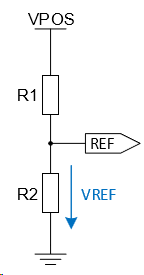
\includegraphics[width=0.2\columnwidth]{Images/widerstandteiler}
	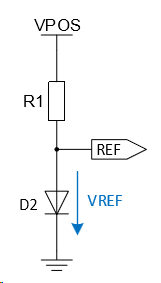
\includegraphics[width=0.22\columnwidth]{Images/widerstandsteiler_diode}
\end{center}
Eine Änderung an $V_{pos}$ wirkt sich direkt auf $V_{ref}$ aus. Um dies zu verbessern wird eine Diode anstelle $R2$ eingesetzt. Mit der Diodenspannung von $V_{ref} = V_D$ wird dies zwar Temeraturabhängig, jedoch hat $\Delta V_{pos}$ weniger einfluss.
\begin{align*}
	I_D &\approx I_S \cdot e^{\frac{V_D}{n\cdot V_T}} \xrightarrow{} V_D = \frac{nKT}{q}\ln\left(\frac{I}{I_S}\right) \\
	I = \frac{V_{pos} - V_D}{R1} &\approx \frac{V_{pos}}{R}
\end{align*}
Das Verhätniss lässt sich nun durch $S = \frac{1}{\ln\left(I/I_S\right)}$ berechnen. Damit ist zwar eine kleine Lastsabhängigkeit, dafür jedoch eine Temp. Abhängigkeit.

\subsection{Bootstrap-Referenz}
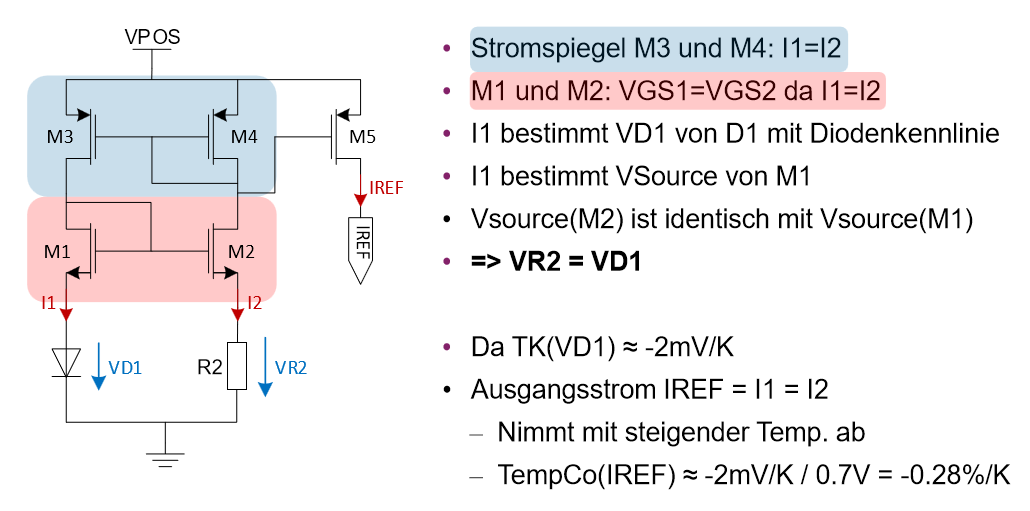
\includegraphics[width=\columnwidth]{Images/bootstrap_ref}
\[
V_{D1} = n\cdot V_T \cdot \ln\left(\frac{I_1}{I_S}\right) = I_2 \cdot R_2 = V_{R2}
\]
Problem bei dieser Schaltung ist, dass sich zwei Arbeitspunkte einstellen können, der ungewünschte bei $I_1 = I_2 = 0$

\subsection{PTAT}
\begin{center}
	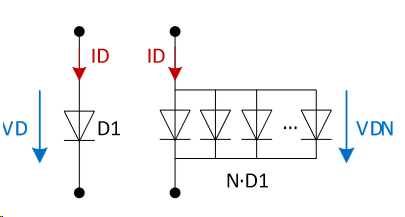
\includegraphics[width=0.5\columnwidth]{Images/pat}
\end{center}
Die \textbf{P}roportional \textbf{t}o \textbf{a}bsolute \textbf{T}emperature Quelle liefert eine $\Delta V_D$ proportional zur absoluten Temperatur $T$.
\[
\Delta V_D = \frac{nkT}{q}\cdot\ln(N) = V_{PTAT} = const \cdot T
\]
Der Temperaturkoeffizient $TK$ bei Raumtemperatur beträgt $\frac{k}{q} = 0.0.86\frac{mV}{K}$. Wenn diese Quelle mit einer Diodenspannung mit $TK = -2\frac{mV}{K}$ kann eine $TK = 0$ erreicht werden. 

\begin{center}
	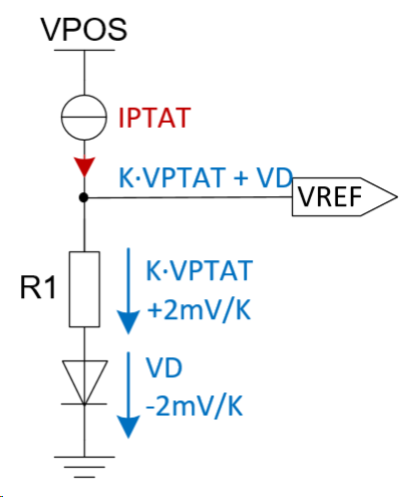
\includegraphics[width=0.3\columnwidth]{Images/ptat}
\end{center}

\subsection{Serie-Referenzspannungsquelle}
\begin{center}
	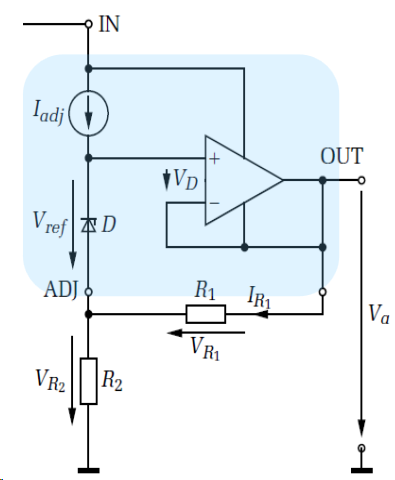
\includegraphics[width=0.4\columnwidth]{Images/serie-refquelle}
\end{center}
Interne Bandgap-Quelle oft $V_{ref} = 1.25V$.
\[
V_a = V_{ref} \left(1 + \frac{R_2}{R_1}\right)
\]